% Modified
\documentclass{l3proj}
\usepackage{wrapfig}
\usepackage{csquotes}
\usepackage{glossaries}

\newglossaryentry{jquery}
{
	name=JQuery,
	description={A free and open source JavaScript library that is used by Web developers to navigate HTML documents, handle events, perform animations and add AJAX interactions to Web pages}
}

\makeglossaries
\SetBlockEnvironment{quotation}
\begin{document}
\setcounter{secnumdepth}{3}
\title{Multi-device Recording System}
\author{Alastair Weir \\
        Gordon Adam \\
        Peter Yordanov \\
        Keir Smith \\
        Georgi Dimitrov}
\date{28 March 2014}
\maketitle
\begin{abstract}

Surrounding us in city life there are unqiue moments missed everyday by experiencing  them through the lens of a smartphone instead of being 'in the moment'. That instance is lost in time and never fully appreciated. The video or images captured are then restricted to that specific person, only able to relive the moment from their limited perspective. By creating a mobile first approach to capturing locational audio centred around these moments, MDRS can offer new insights and crowdsource distinctive, new  perspectives of life in our cities. This aim was successfully achieved with a functioning web and mobile application to allow users to gather this information while still enjoying the moment, then later explore their perspective and others in a unique way. Our testing has shown...

\end{abstract}
\educationalconsent
\tableofcontents
%==============================================================================
\chapter{Introduction}
\label{intro}

\section{Motivations}
Around the world, ubiquitous connectivity is giving users a new avenue to make their voices heard and share their stories. With MDRS (multiple device recording system) we leverage a mobile device’s sensors and give everyone a platform on which share their story, or experience, in a specific place and time. These all join to form a map where others can explore and listen to these experiences synchronously in chronological order. If more than one recording happened in the same area at the same time they will playback together, melding to create an unique and richer insight into an event such as a concert.

In recent years concert attendees have derided a rising trend of viewing an amazing live performance, happening mere metres away, through a sea of smartphone screens in front of them. These screens detract from an attendee's enjoyment to the extent some bands ask their fans to not use their phones during their performance. MDRS is a step beyond this frustration as it's passive, letting a user record clips of the concert to share with their friends later while their phone is still in their pocket. This frees their attention to immerse themselves in what is happening. Users can actively improve the experience of the concert for everyone while still creating something they can share with friends later.

MDRS could also be used in law enforcement and political movements. It's unique storytelling ability to combinine the spoken word and images while communicating an accurate sense of place sets it apart from alternative methods. By giving an investigator multiple perspectives to an incident, they can ensure that a fair judgement is passed. If a victim is struggling to find justice they can effectively ‘crowd-source’ their evidence from those who are present. This would help to keep political protesters safe and protect their rights when dealing with law enforcement. MDRS gives a voice to unheard or mistreated minorities.

In the case of a festival, bands could upload their own recording of their performances with professionally captured images and the location of their stage within a festival site. These uploads could create a concentrated virtual space populated with dozens of  professional recordings and the crowd’s experiences for users to explore and gain a noteworthy perspective they might have missed at the time.

These use cases are a slice into the motivation that drives this innovative project. They demonstrate a rare opportunity to leverage some of the vast data our smart devices are capable of capturing from the physical space and generate something original.

\section{Aims}
As more connected mobile devices reach the hands of consumers, billions of pieces of data are being created every day. A lot of this data centres around events in people’s lives from large scale political movements ranging from the Arab Spring to a friend’s birthday party. Extracting meaning from these colossal stores of data created by this internet of things is one of the key challenges in technology today.

MDRS aims to allow people to easily share experiences and moments important to them through a combination of location, audio recordings and images. We aim to leverage Android as the dominant mobile platform around the world. This gives a large install base with many possible uses for MDRS instead of catering to a narrower user type. The app should be able to passively record in the background allowing its user to actively participate in the event happening around them. This removes the conscious decision to become a passive documenter instead of participating in what is happening.

A web application will allow users to explore the recordings uploaded in an interactive map. They will be able to search for specific events or select all recordings in an area for synchronous playback. By achieving this unique playback style accurately synchronised in time, MDRS offers a more meaningful way to explore data than listening to recordings individually. We aim to surprise and inform our users by offering them insights into different cultures, walks in life or new perspectives on events in their own lives. We believe the service should be free to use and access, offering a simple and attractive interface accross it's two platforms.

\section{Background}
Mobile was an interest in many of the team members and a trending sector in the technology industry. These devices have surpassed the use of computers in the home and are of particular interest to UI/UX designers. Their screen sizes, use cases and interaction models are very different to traditional devices and developers are constantly finding new innovations in this field. With the proliferation of wearable devices such as smartwatches, leveraging the sensors within these powerful devices is an area of intense interest. Android’s support for varied screen sizes and device types gives the team a welcome technical challenge while leveraging existing our existing knowledge of Java.

Designing for the web incorporates numerous markups, programming languages and libraries. This makes for a steep learning curve but by leveraging previous experience and through other coursework undertaken throughout the year, acquisition of the required skills becomes much easier. To build a lightweight web client means leveraging core web technologies such as HTML and CSS to their fullest to improve the user’s experience as much as possible while keeping the application lean and fast. Where needed Javascript is used to add more dynamic features desired to the project.

Deploying a web application can be done in many different ways with innumerable frameworks and tools available to use. Again, hoping to use pre-existing skills we researched and chose the Python based Django framework as the basis for MDRS’ backend. Its versatility made it an ideal choice while not adding to the heavy workload the project demanded with another new language to learn.

Today in the market, very few systems similar to MDRS can be found for use. Services such as Soundcloud or Audioboo allow the user to easily record audio and upload it to a website for sharing but beyond that offer limited functionality. These both heavily focus on the social interaction around each recording. Software such as Audacity would allow the user to manually stitch the audio together but this process is technical and time consuming.

The only product that matches more of MDRS’ aims is Broadcastr. A New York City based startup now renamed SPUN released Broadcastr in 2010, allowing users to record stories and link them to a static location. The app gained media attention upon release with recommendations from the BBC and Wired. SPUN later abandoned the project and moved into geo-targeted advertising. While similar, Broadcastr still differs as MDRS allows for a recording to forge a path across the map, linking the audio and images to a user’s location as they move through a place.

\section{Preliminaries}
To fully understand this dissertation, the following knowledege would be beneficial:
\begin{itemize}
\item A basic understanding of the construction of an Android application
\item A basic understanding of how Django projects function
\item Syntactical understanding of Java, Javascript and Python
\item Willingness to follow the links to the various resources used as part of MDRS
\end{itemize}

%==============================================================================
\chapter{Research}
\label{Research}

With the idea of the potential for MDRS, it was key for the team to research key features and tools they hoped to integrate into the project and to find things that would fit well into our imagined product.

\section{Technologies}
\subsection{Timeline}
The use of a timeline of recordings was central to MDRS' interation conceit. TimelineJS offered an attractive UI populated with clear boxes for each event that when clicked on, centred the timeline to that element and associated metadata would be displayed above it. It was found to be effective in clearly communicating the difference between recordings, portraying a vertical line on the timeline for each event. The metadata view above the timline, while unnecessary for the front page, would be crucial for the user's profile view. Importantly for MDRS, this timeline is also well supported on mobile devices.

\begin{figure}[ht!]
  \centering
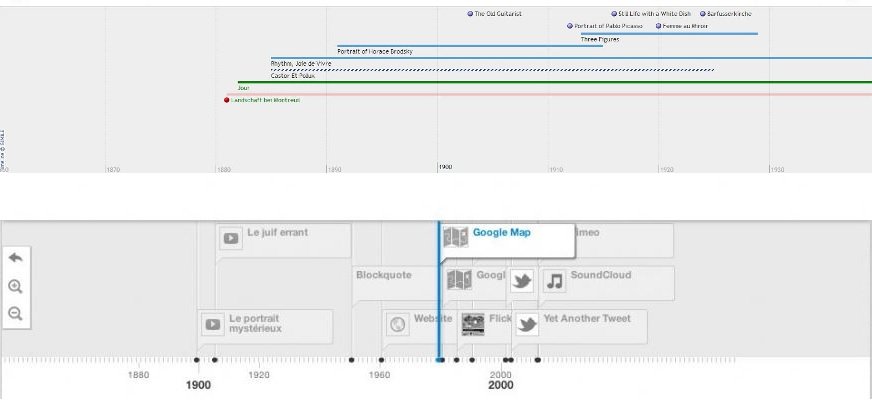
\includegraphics[width=0.75\textwidth]{images/similie_knightlab_timeline.jpg}
\caption{MIT's SIMILIE Timeline (top) Knightlab's Timeline JS (bottom)}
\end{figure}

Another timeline that was researched was the SIMILIE Timeline, developed by MIT. The main point of contention with this timeline is in it’s appearance, which falls much further short of it’s contenders. There was also some questions about it’s compatibility with Internet Explorer and mobile devices. The upside however is that it offers a greater level of customisation, allowing much more flexibility with it’s styling.

After a comparison TimelineJS was chosen due to its ease of use for the end user and its attractive user interface which was deemed a more important feature than greater customisability. Also the compatability issues of the SIMILIE timeline could have caused problems further down the line, which we may not have been able to resolve.


\subsection{Map}
OpenStreetMap was thoroughly researched. It's open source roots and excellent level of detail and accuracy was attractive. When combined with a Javascript library such as Leaflet, the potential was excellent. It’s downfall lay in the fact that we would have to store the raw map data, which uncompressed could comprise up to 400GB. Storing this on our server would be an impossibility. And while Leaflet would support our central aims, its limited functionality restricted the possible direction the team could take MDRS in. The default style for OpenStreetMap was also far more detailed, reducing readability and cluttering an interface we aimed to keep simple.

\begin{figure}[ht!]
  \centering
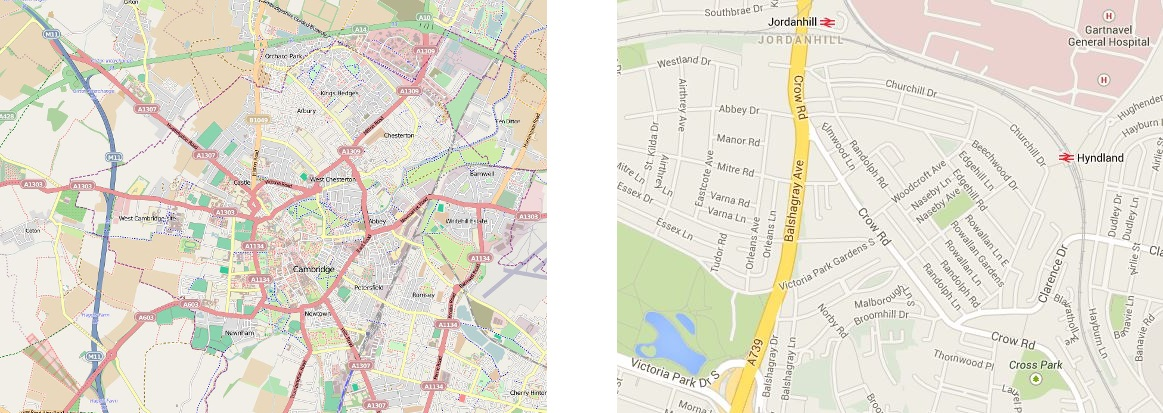
\includegraphics[width=0.75\textwidth]{images/openstreetmap_google-map.jpg}
\caption{OpenStreetMap (left) Google Map (right)}
\end{figure}

Google Maps was seen as an strong alternative. While it was not open source, it offered comparative quality. A weakness found in the limitations set on the free use of the API. It was discovered that after the obtaining of an API key however we would have access to 25,000 user visits a month. It was decided this limitation would not affect MDRS in its early stages. The default map style for Google Maps was far more simplistic  fitting more neatly with our designs. The API documentation for Google Maps was also excellent giving many examples and walkthroughs which would help make development considerably less confusing.

Taking these points into account it was decided that we would use Google Maps as no extraneous data would be stored on our server and the API appeared to be easier to use as well.


\subsection{Front-End Web Framework}
PureCSS is described on its website as,

\blockquote{“A set of small, responsive CSS modules that you can use in every web project.”}

This was an ideal candidate for our front-end framework as it was minimalistic in both size and appearance with the entire set of modules coming in at only 4.5KB (compressed). The documentation for PureCSS was also extensive which would help to ease problems during the development process of the front end.

Twitter's Bootstrap framework appeared to be a more complete solution. It provides icons, styling, and a number of UI elements ready to be easily added to a webpage. However in being the complete package, less flexibility would be offered in the appearance and the front end could end up having very little of it’s own character. Performance also suffers due to the size of the Javascript and CSS files needed. The documentation with Bootstrap was also very detailed, appearing to be more extensive than that provided with PureCSS.

PureCSS was chosen in the end as it was far more lightweight and met our simple requirements. It gave a solid foundation on which to build our website from. Although Bootstrap is powerful it would have complicated our application unnecessarily.


\subsection{Audio Playback}
Buzz is a JavaScript library that utilises the HTML5 audio element. This library worked well grouping multiple audio files together and playing them simultaneously.

JPlayer was also considered though it had drawbacks in playing multiple files as there appeared to be no obvious way to play multiple files without having multiple instances of the player UI. This had the potential to negatively impact performance in a big way. The JPlayer's unattractive, heavy UI would also have to be repeatedly used within our interface.

The team took the decision to use the Buzz JavaScript library as it was exactly what we were looking for on this particular occasion.

%==============================================================================
\chapter{Planning}
\label{Planning}

Plans in here will come in handy

\section{Use Cases}
Before starting the actual implementation of the application features, we thought of, and documented, the possible use cases of the system in the form of paper-drawn user stories. These blossomed into situations that MDRS could actively improve a user's experience giving us a grounding from which to work from.

<paper user stories images>

\subsection{Recording at a Demonstration} The synchronisation of multiple audio streams at a protest or any other type of public demonstration would enable the listener to hear different perspectives of the demonstration. What is more, they can switch between the source audio streams in order to distinguish speech, conversations, etc.

Scenario: John is a lecturer at a public protest in Glasgow regarding the academic salaries in the UK. He is at the protest with a couple of friends - Jane and Chris, who are also a part of the academic society. However, the protest has not managed to attract that many people and there has been no effect to date.

The three friends are trying to attract their colleagues by installing the MDRS mobile application on their Android cellphones and recording conversations while at the protest. Then sharing the different views people express in their statements from multiple vantage points at the protest can be listened to by their fellow lecturers, tutors, etc. - members of the academic community in Glasgow in order to make them realise the need to take part in the event and try to change their lives for the better.

\subsection{Audio Syncronisation at a Music Festival} Being able to synchronize multiple recordings from a music festival for instance is also a possible use case for this application. It will give end users the opportunity to listen to the music event as if they attended it considering the various vantage points used for audio recording. Also, noisy audio streams can be switched off to improve the audio quality of the playback.

Scenario: There is a music festival on a statium in London and Tom (from Aberdeen) and Kate (originally from London), who know each other, have bought tickets and are going to attend the festival. However, they are not going together and do not know that are both going to be attending. Tom has a ticket for the front rows because he has been expecting to see his favourite band live for months, while Kate is there just for fun and has grabbed herself a cheaper ticket somewhere in the back.

They are both recording the event using the MDRS mobile app to upload it to their personal timeline later.

After the event, meet each other by accident and talk to each other about how they are getting on with their lives. After uploading the recordings they made on the festivel online, with the MDRS web application they will be able to compare/ switch between the audio streams and listen to both of them at the same time - the louder and clearer recording Tom made and the more noisy one Kate recorded.

\subsection{Home Party Recording} The multi-device audio system can also be used for other entertainment purposes, such as recording conversations from different locations at a house party. Synchronized playback ofthe audio will be great fun to listen to on the next day after the party.

Scenario: John is hosting a house party and everyone starts recording people’s conversations with their mobile devices scattered around in the rooms.

The next day after the fun is over, it is going to be greatly entertaining to listen to all the gossip people have been discussing.

\subsection{Sports Event} If there is a sports event such as a championship or a tournament which involves matches being played on numerous locations at the same time, it would be nice to be able to record commentators discussing the game and synchronizing their statements to keep track of the present result.

Scenario: Mark is a great fan of tennis and is attending the tennis tournament in Dubai in 2012. He idolises Rafael Nadal and has bought tickets for his tennis match against Novak Djokovic, court 1. At the same time, however, on court 4 plays Roger Federer against Grigor Dimitrov.

Mark is a very keen supporter of the young Bulgarian rising star but cannot be at that court at the same time. By using MDRS to record the match on court 4, one of Mark’s friends who is also attending the tournament but has a ticket for the other section is able to deliver Mark the audio stream from the other tennis court, making it possible for mark to listen to judges on both courts to keep track of the result.

\section{MoSCoW requirements}
Listed below are the project functional requirements the team identified with their priority rating based on the MoSCoW system:

\subsection{Must Have}
	Web application:
		- the system needs a website with a backend support for audio processing

	Mobile application:
		- the system also comprises of an Android application for audio capture to be submitted to the database of the website via an upload form

	User Authentication:
		- potential users need to be able to register on the web application in order to keep track of each person's individual audio recordings and visited locations

	Recording audio:
		- the system mobile application needs audio recording functionality so that the user could quickly capture audio with the click of a button

	Recording submission:
		- interaction between the Android app and the webapp

	Storing audio recordings:
		- the mobile app needs to store recordings on the server for processing

	Audio synchronisation:
		- audio synchronization functionality on recording selection

	Recording timeline:
		- a timeline to show database recordings based on their start and end time (as well as provide a temporal visualisation of overlapping recordings)

\subsection{Should Have}
	Playback selection:
		- users need to be able to listen to all the recordings and be able to select

	Geo location:
		- the system needs to store current user location


\subsection{Could Have}
	Route tracking:
		- once a user has started recording, the system needs to use GPS tracking to update current location and save it to the database when recording activity has finished

	Taking photos:
		- the Android application needs to enable the user to take photos while recording to make the playback experience more realistic and detailed

	Filter recordings depending on times:
		- a nice feature will be to provide users the option to filter recordings and display only those from a specific time period on the map and the timeline

\subsection{Would Have}
	User account enhancements:
		- it would be nice to provide users the opportunity to change their avatar

	Recording grouping in events:
		- after uploading a recording it would be a nice feature to provide the option of creating an event as a property of the recording object or selecting one from the list of events that have already been created

	Recording tags:
		- users could add relevant tags to their recordings which will enable easy search and recording filtering


\section{Project Timeline}

From the outset, the team laid out a flexible timetable for the project, accounting for the series of phases a project must undergo.

During week one we filled the consent forms which were distributed to us after the group allocations were announced and submitted the ballot.

We had a couple of days to make a final decision on the final six projects from all the project proposals and created a Facebook page to help with the communication between group members in general and more specifically, as a form for project management beside the RedMine project management system we decided to use as a primary one.
After we understood the team project allocation, we started researching and planning about the key functional requirements how we are going to implement them, consulting the project supervisor on how to approach each design and implementation phase.

Having organised a couple of team meetings, we exchanged contact information and made a final decision on the system for version control and project management - Github and RedMine accordingly. Following a quick discussion we also took the decision to use the agile framework for the team structure and chose Keir as our scrum master.

After submitting the organizational document on Moodle we met with the project supervisor and asked questions about server space, user interface structure and basic requirements explanation in general. Not long after that meeting we had our own development server provided by the university.

For next week at the start of November we were all designing sample user stories in the form of comic story boards to present on the supervisor meeting. The whole month (October) was devoted to requirements interpretation, planning and design - decision making in general.

The following couple of weeks were spent thinking of user interface ideas/mock-ups for the web and mobile application. Some quick sketches where prepared which we presented on the supervisor meetings. We also set up our GitHub repository and as most of us had not used it before, started making test push, pull, commit, etc. commands to familiarise ourselves with the version control system.

We started thinking about what technology our project is going to utilise and how to implement the key features we had identified. One of the main tasks was to make a decision on audio time synchronisation, which could be done in a number of ways; a great deal of research had to be undertaken before making a final decision. A possible option was to use an NTP - network time protocol with a reference clock. Other viable options were GPS clock synchronisation or OS clock synchronisation. NTP was chosen as it seemed the most reliable and easy to implement option.

At the end of October we decided to make a choice on the web middleware framework for our project. The main candidates were Django (Python based) and the SPRING (Java oriented) development frameworks, both of which are well designed, simple to understand and make code maintainability very efficient. After considering the pros and cons of the two frameworks, we chose to use Django as it seemed to be better documented and would perfectly suit the needs of the multi-device-audio project web application. Apart from that, we also knew that our coursework and material in the second semester’s Distributed Information Management 3 course would require us to learn how to use Django, further strengthening our choice.

We spent the next couple of weeks familiarising ourselves with the framework and testing various tutorials using the 'Tango with Django' online book which is a through guide containing a lot of detailed information with useful design and feature implementation techniques included.

We organised group meetings a two to three times a week in order to make plans about the database schema and the application flow of control. After reaching final decisions on these matters, we set up the database classes and created a population script using the tutorials from the book in order to test that everything is working as expected. Also designed the project logo prototypes and started to think more thoroughly about the system’s user interface.

The work continued as we divided the functional requirements into bite-sized smaller chunks and different group members were allocated different tasks with set deadlines which were all monitored on RedMine.

\textbf{<GANTT chart from RedMine, GitHub activity diagram>}




%==============================================================================
\chapter{Design}
\label{design}

The core of our design sprung from early storyboarding and imagined user
profiles which informed us extensively to what a possible system might look
like. Each team member chose a different scenario which they thought MDRS could be used and created a visual aid to describe the user's experience as they interacted with it. As previously discussed, MDRS was viewed as a tool to democratise access to moments through an interactive medium. Storyboards served as an excellent tool to realise the potential of the project and its uses in such varied settings as public safety, political protests, music concerts and disaster areas.

\begin{figure}[ht!]
\centering
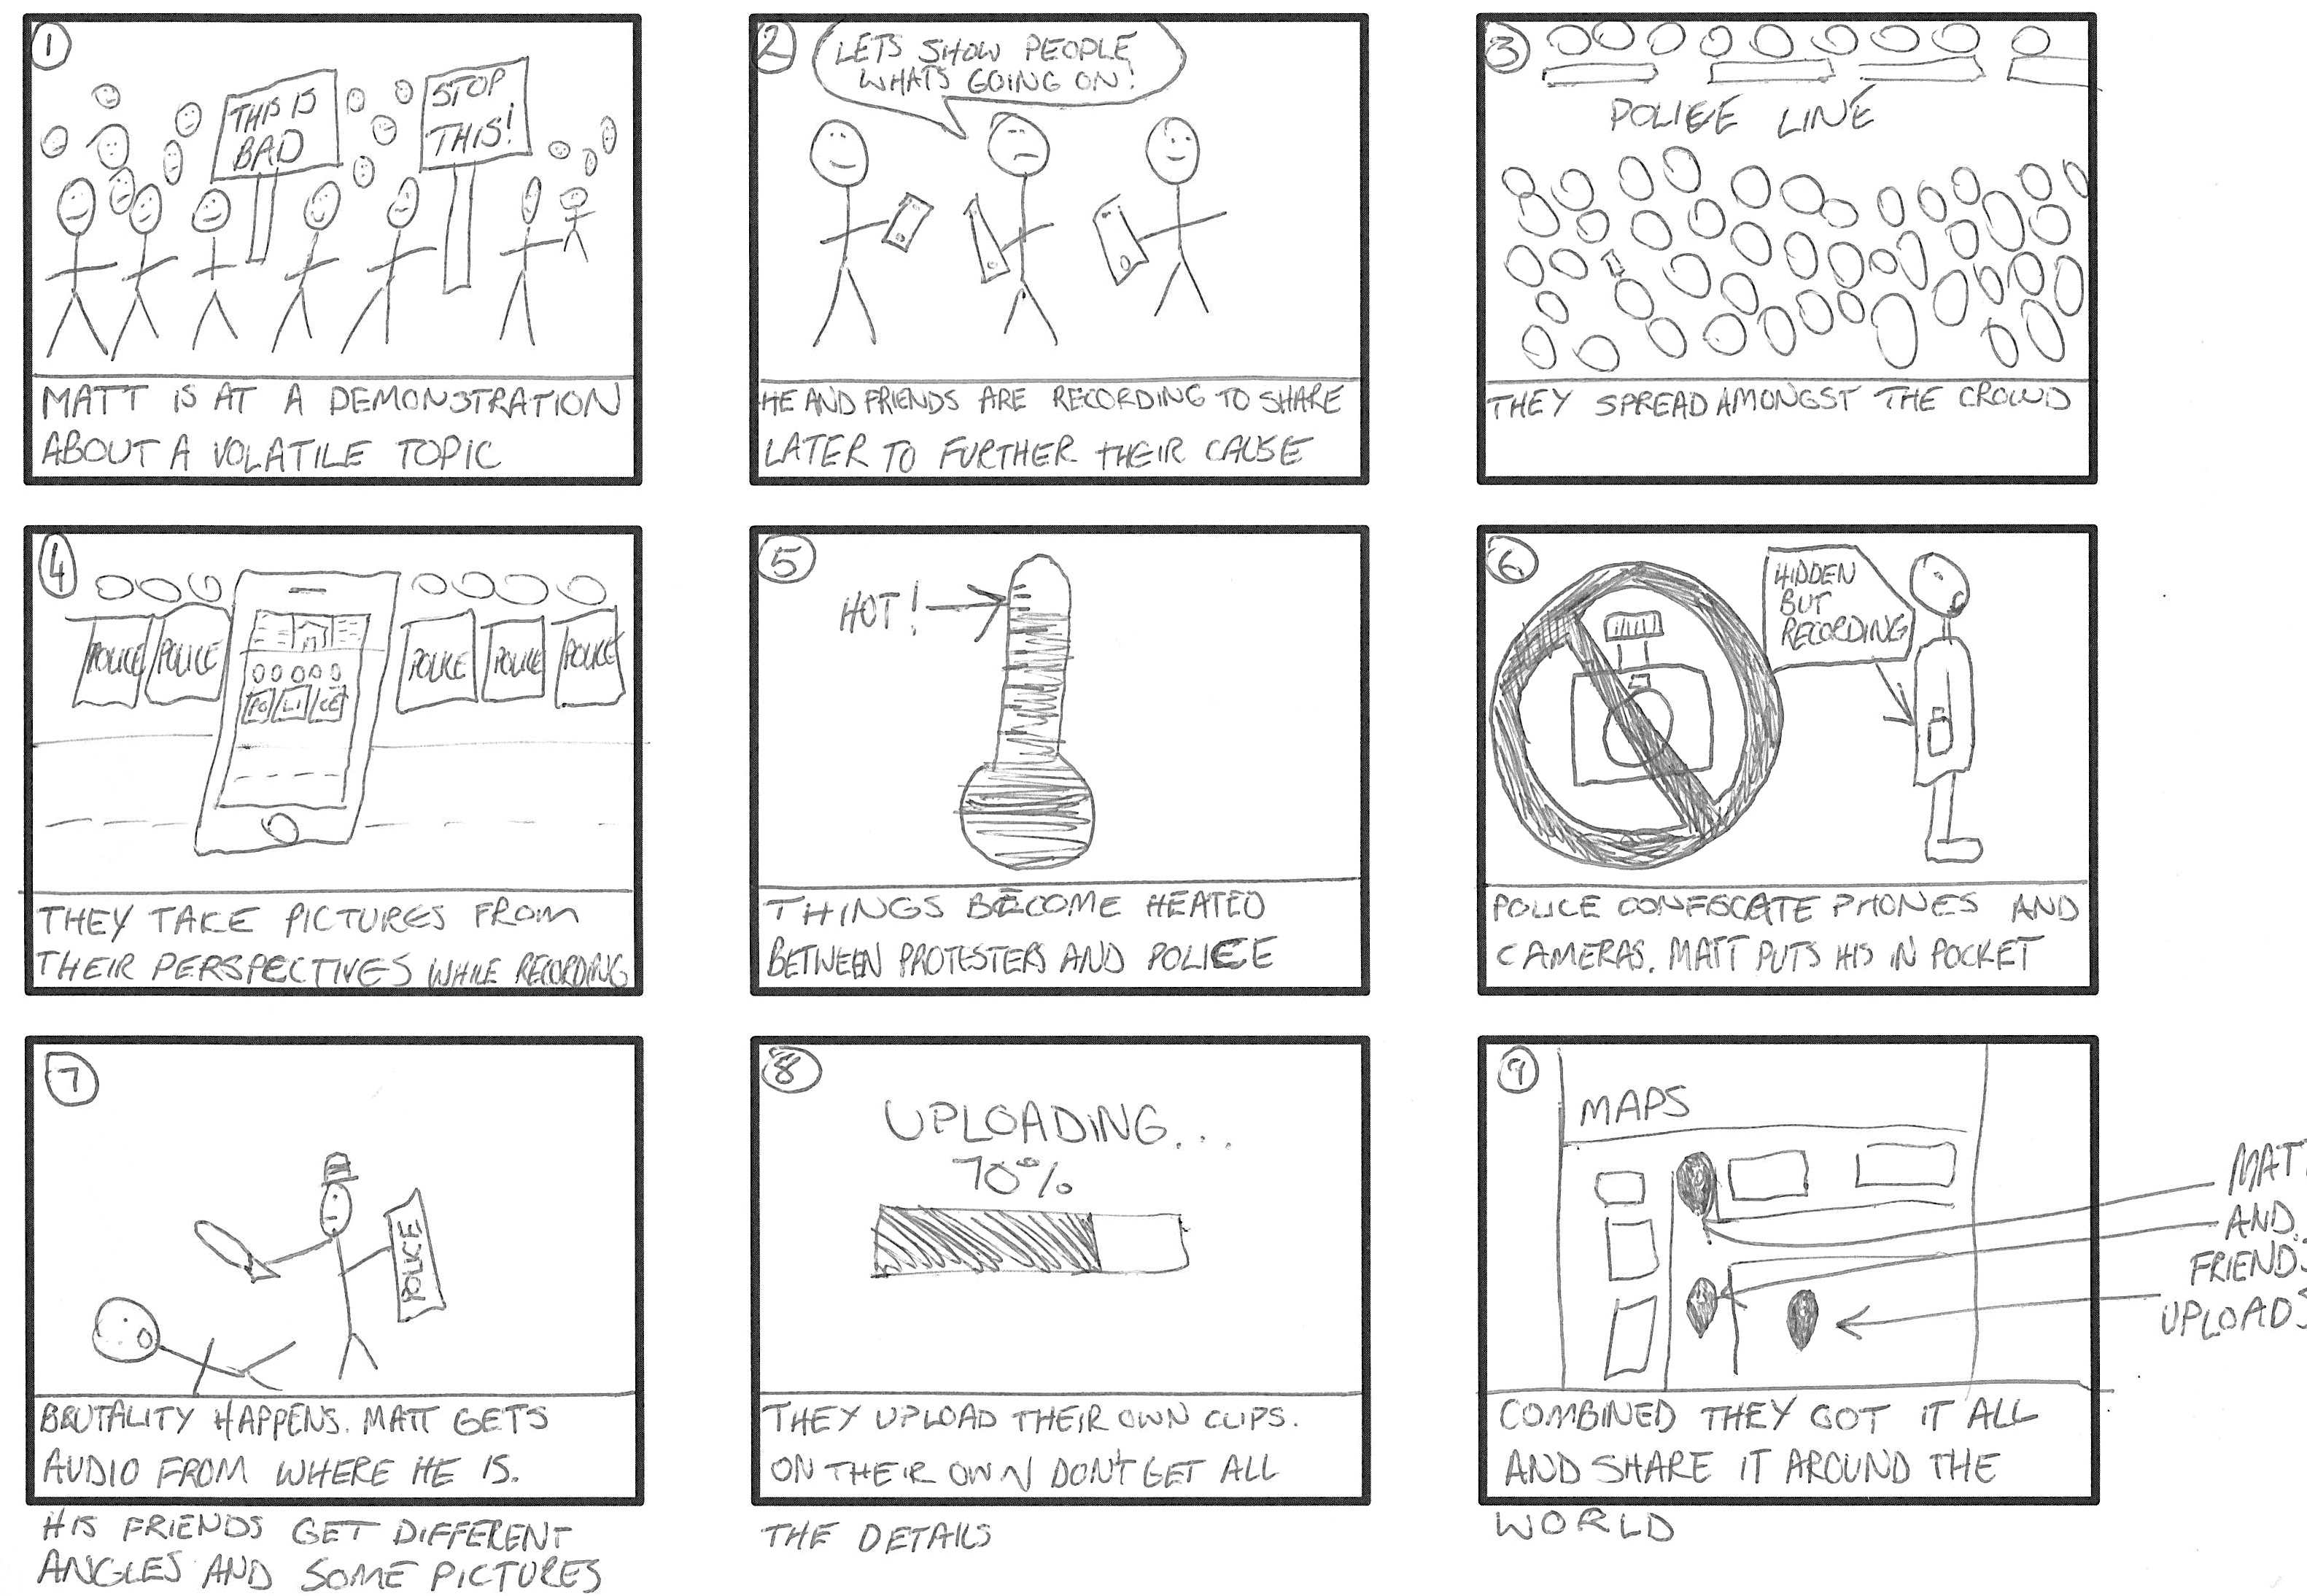
\includegraphics[width=0.75\textwidth]{images/ally-storyboard.jpg}
\caption{An initial storyboard for MDRS.}
\end{figure}

The project's use in public safety was of particular interest to the team. MDRS could serve as an equaliser offering a non-invasive and non-threatening way for police officers to monitor their patrol. It could hold the officers and those they interact with accountable in a alternative way to current methods such as mounted video cameras.

Include another storyboard here {\bf bold}

From our storyboards we realised that MDRS should be more than an audio recorder with location tracking. By allowing the user to capture images, we could combine these three sources of information into a virtual environment that other users could explore.

\section{User Interface} The realisation that the project would be spread across
both mobile and static devices raised the need for two interaction models for
MDRS was found quickly. For capturing the various forms of data a mobile
implementation was key. Android was quickly chosen as the frontrunner for its
proliferation in the market, an expected ease of development due to its Java
base, which much of the team had experience in, and access to test devices
amongst the team. A web application counterpart was planned for the flexibility
of web technologies which allowed a wide variety of devices and users to access
this facet of the project rather than a native application for any given
Operating System would.

\subsection{Web Application}   Given the nature of MDRS, the team look to the
Distributed Information Management course taught in second semester as a source
of possible tools. Taught by Leif Azzopardi, the course is structured around the
use of Django, a Python based web framework which would offer us the flexibility
to create a rich, dynamic application easily deployable and widely available to
possible users. Widely used, Django had a wide range of support materials
available including Tango with Django written by Azzopardi and Glasgow
University postgraduate David Maxwell. This resource and knowing we would have
to learn it later through coursework made the framework choice an easy one.

\begin{figure}[ht!]
\centering
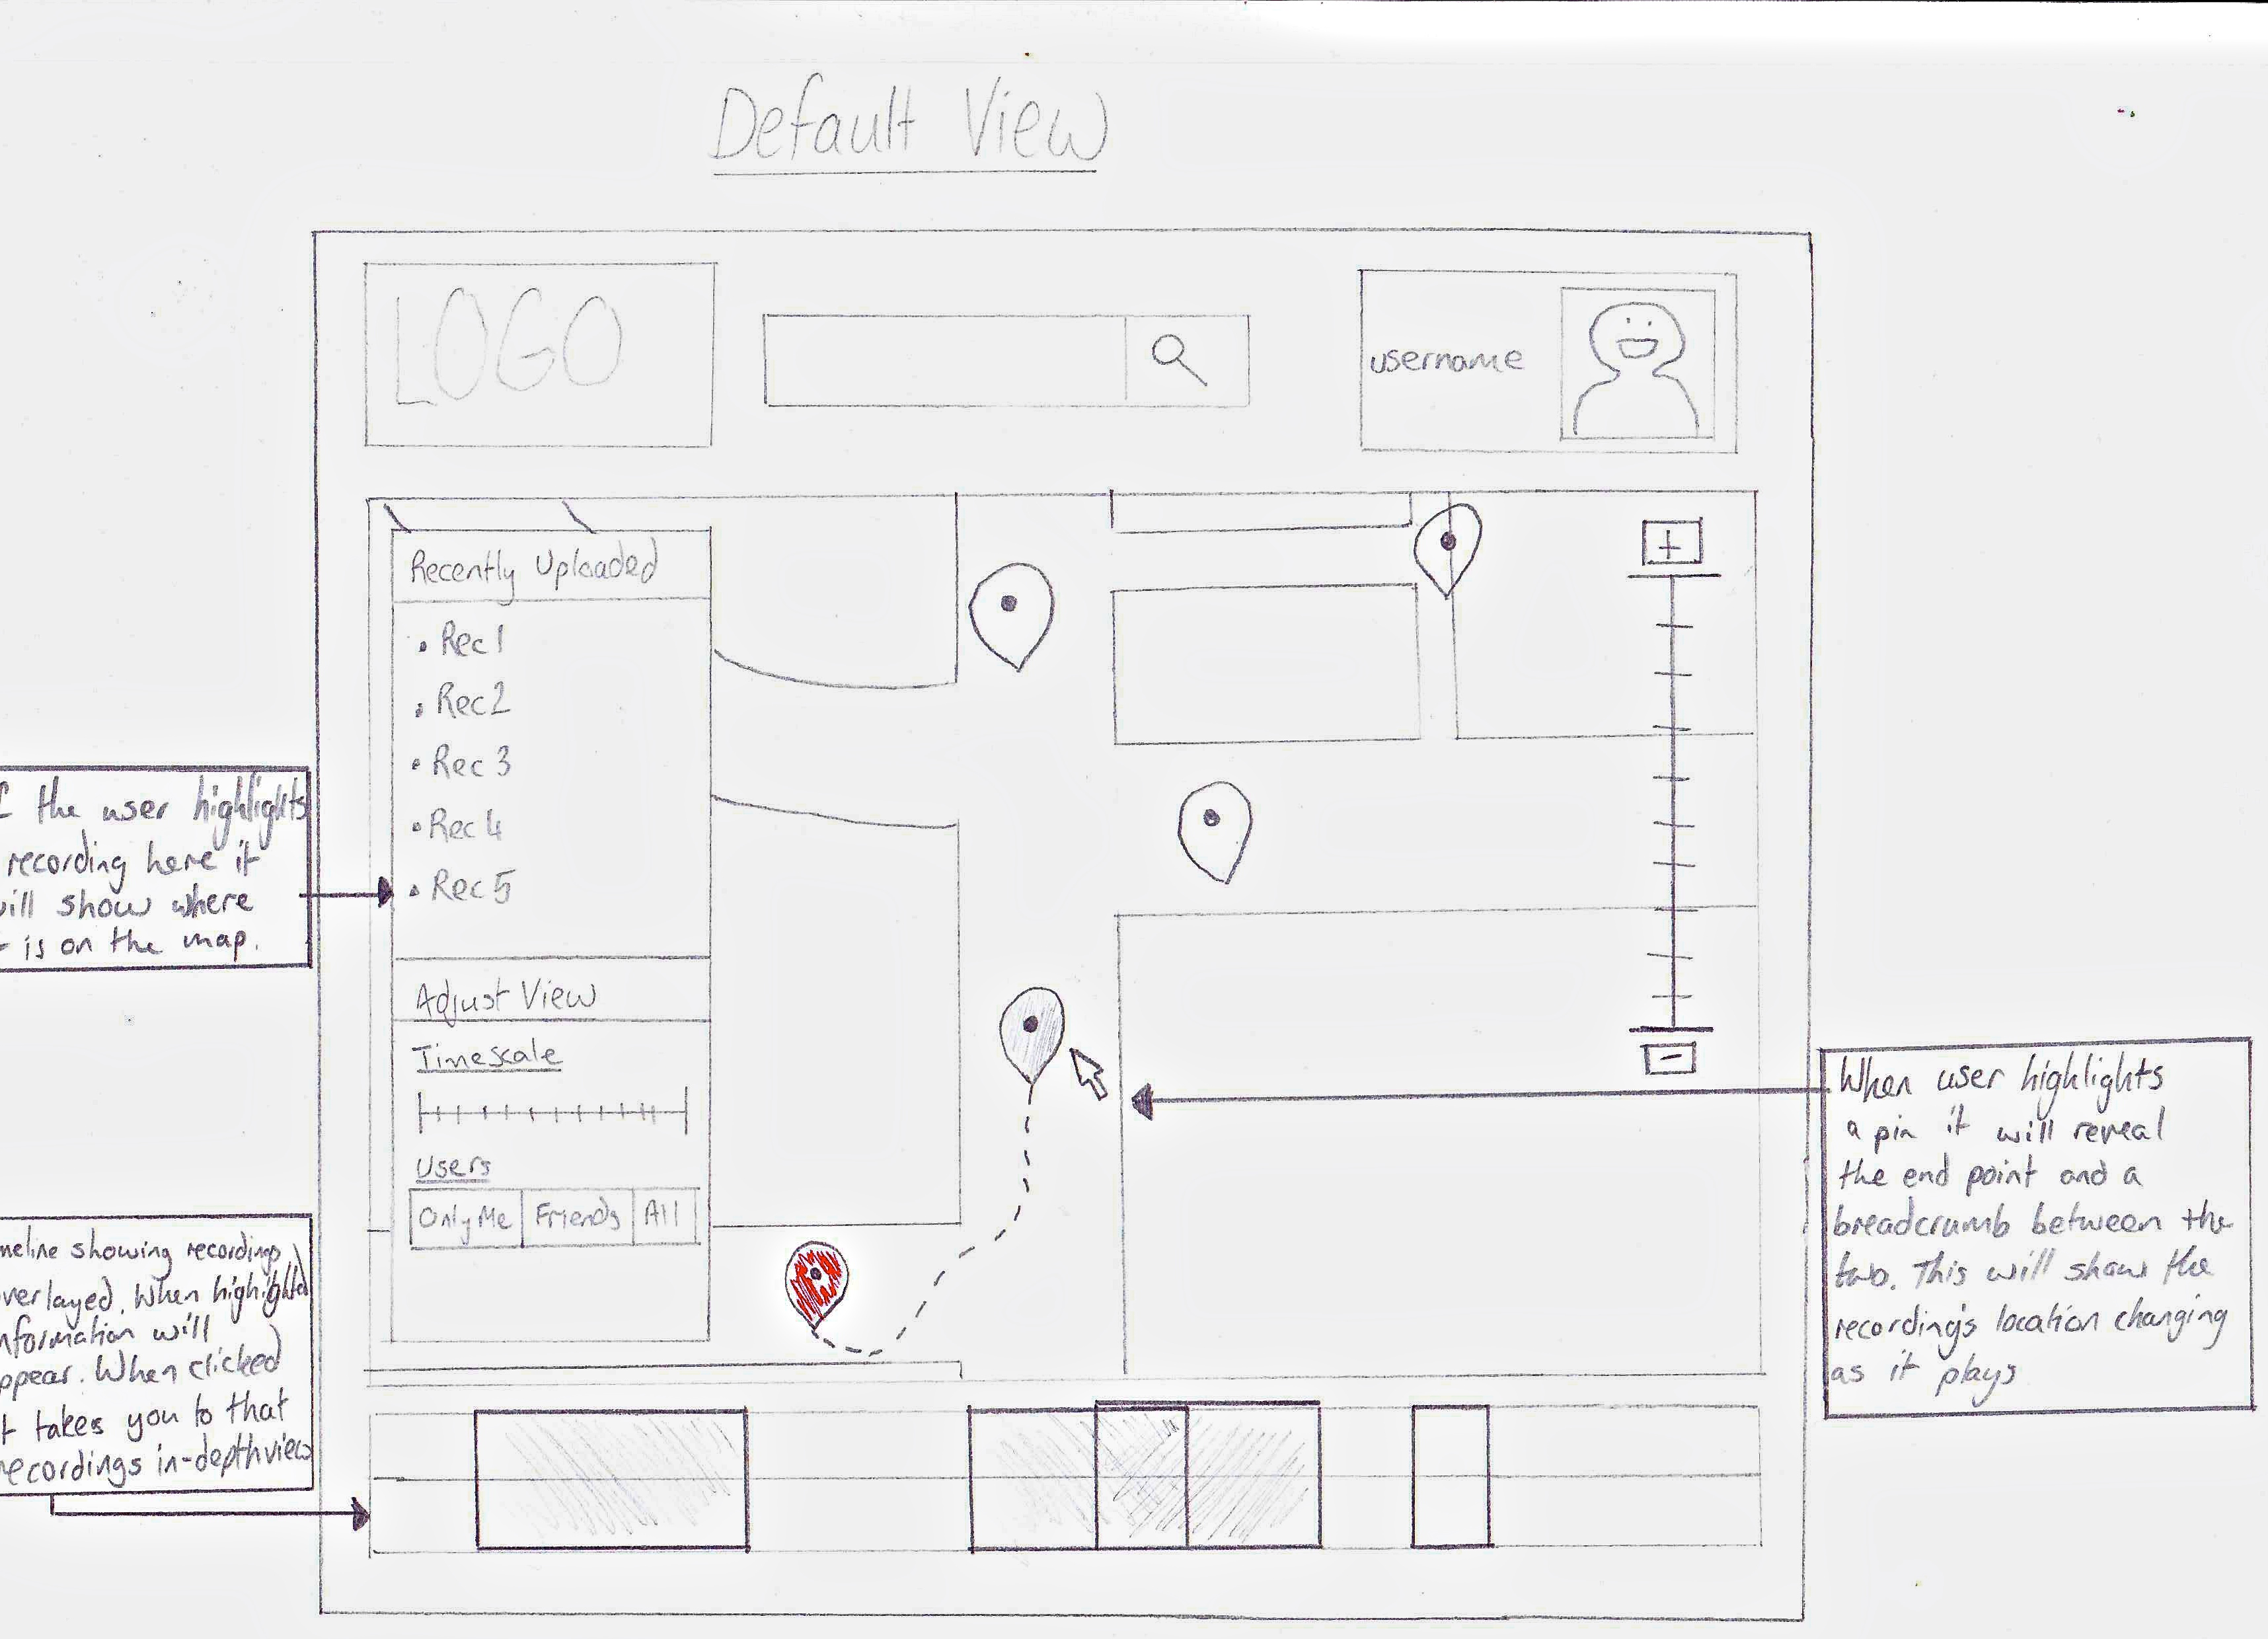
\includegraphics[width=0.75\textwidth]{images/web-map-view.jpg}
\caption{Prototype of map view.}
\end{figure}

The key interaction between the user and MDRS is location therefore it made sense to make a map the central interface. The user would be able to explore the map and click on pins representing recordings. This would then project the path of the recording, indicating where images were captured along the way. Users could then play it back individually or select multiple recordings for synchronous playback. With such an important role, the choice of which mapping API to leverage was extensive in the early stages of the project.

Initially the team were attracted to OpenStreetMap with the very lightweight Javascript library Leaflet. This would give us unlimited access, as the maps were open source, but would require us to host the map tiles which amounted to multiple gigabytes depending on the level of detail chosen. Other disadvantages were the additional difficulty in initial configuration and setup. Another option was Microsoft’s Bing maps which didn’t require as much configuration but were more limited in their free level of access. As an alternative Google Maps was chosen for its simple API and reasonable access for free users. Ultimately is offered 100,000 map loads a month for free. We estimated for a typical user spending 15 minutes on the website that 4 map loads would be needed making this a workable figure for at least 25,000 user visits a month.

Alongside our use of maps, early on in development we prototyped a version which would incorporate Google's Street View. This would allow the user to follow a recording's location trail even more closely. By harvesting the orientation of the recording device we could show where they were looking, showing the Street View at that angle, and overlay any of the user's own images they captured on top of this. While this immersed the user even deeper into the recording, it was unfortunately not taken beyond this prototype stage due to the complexity of implementation.

\begin{figure}[ht!]
\centering
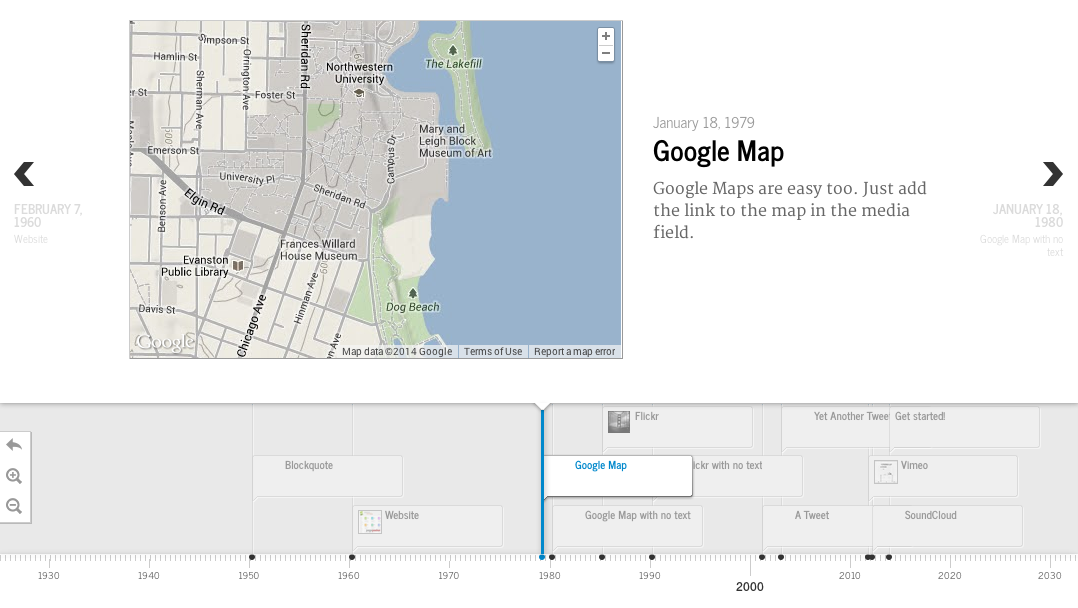
\includegraphics[width=0.5\textwidth]{images/timeline-example.png}
\caption{An example of TimelineJS by KnightLab.}
\end{figure}

A second key component to this interface is the interactive timeline. This was hoped to show the length of each recording and where they overlapped. Upon clicking on one a dialog would show its metadata such as name, description, the user who captured it and accompanying images. Early prototypes also show the ability to move the current position of playback along the timeline to skip to different positions. This level of manipulation was simplified upon selection of TimelineJS which we used to construct it.

Early web interface designs featured a prominent header bar and a floating menu panel which floated over the map. From early prototypes and wireframes this was realised to waste a lot of screen real estate, detracting from the reason the user was on the website. The header bar in particular became wasteful as the ability to search all recordings was downgraded in importance within the application. Through discussion in the team it was decided that users would more likely be interested in audio based on location (the key paradigm of MDRS) rather than searching through keyword. It gave us a stretch goal to aim for if development moved along smoothly. Upon research into interface frameworks the CSS library, PureCSS, was found as a replacement to create an engaging and simple menu interface. Its simplicity favoured our team’s limited prior experience with web design and it’s accompanying documentation is excellent.

\begin{figure}[ht!]
\centering
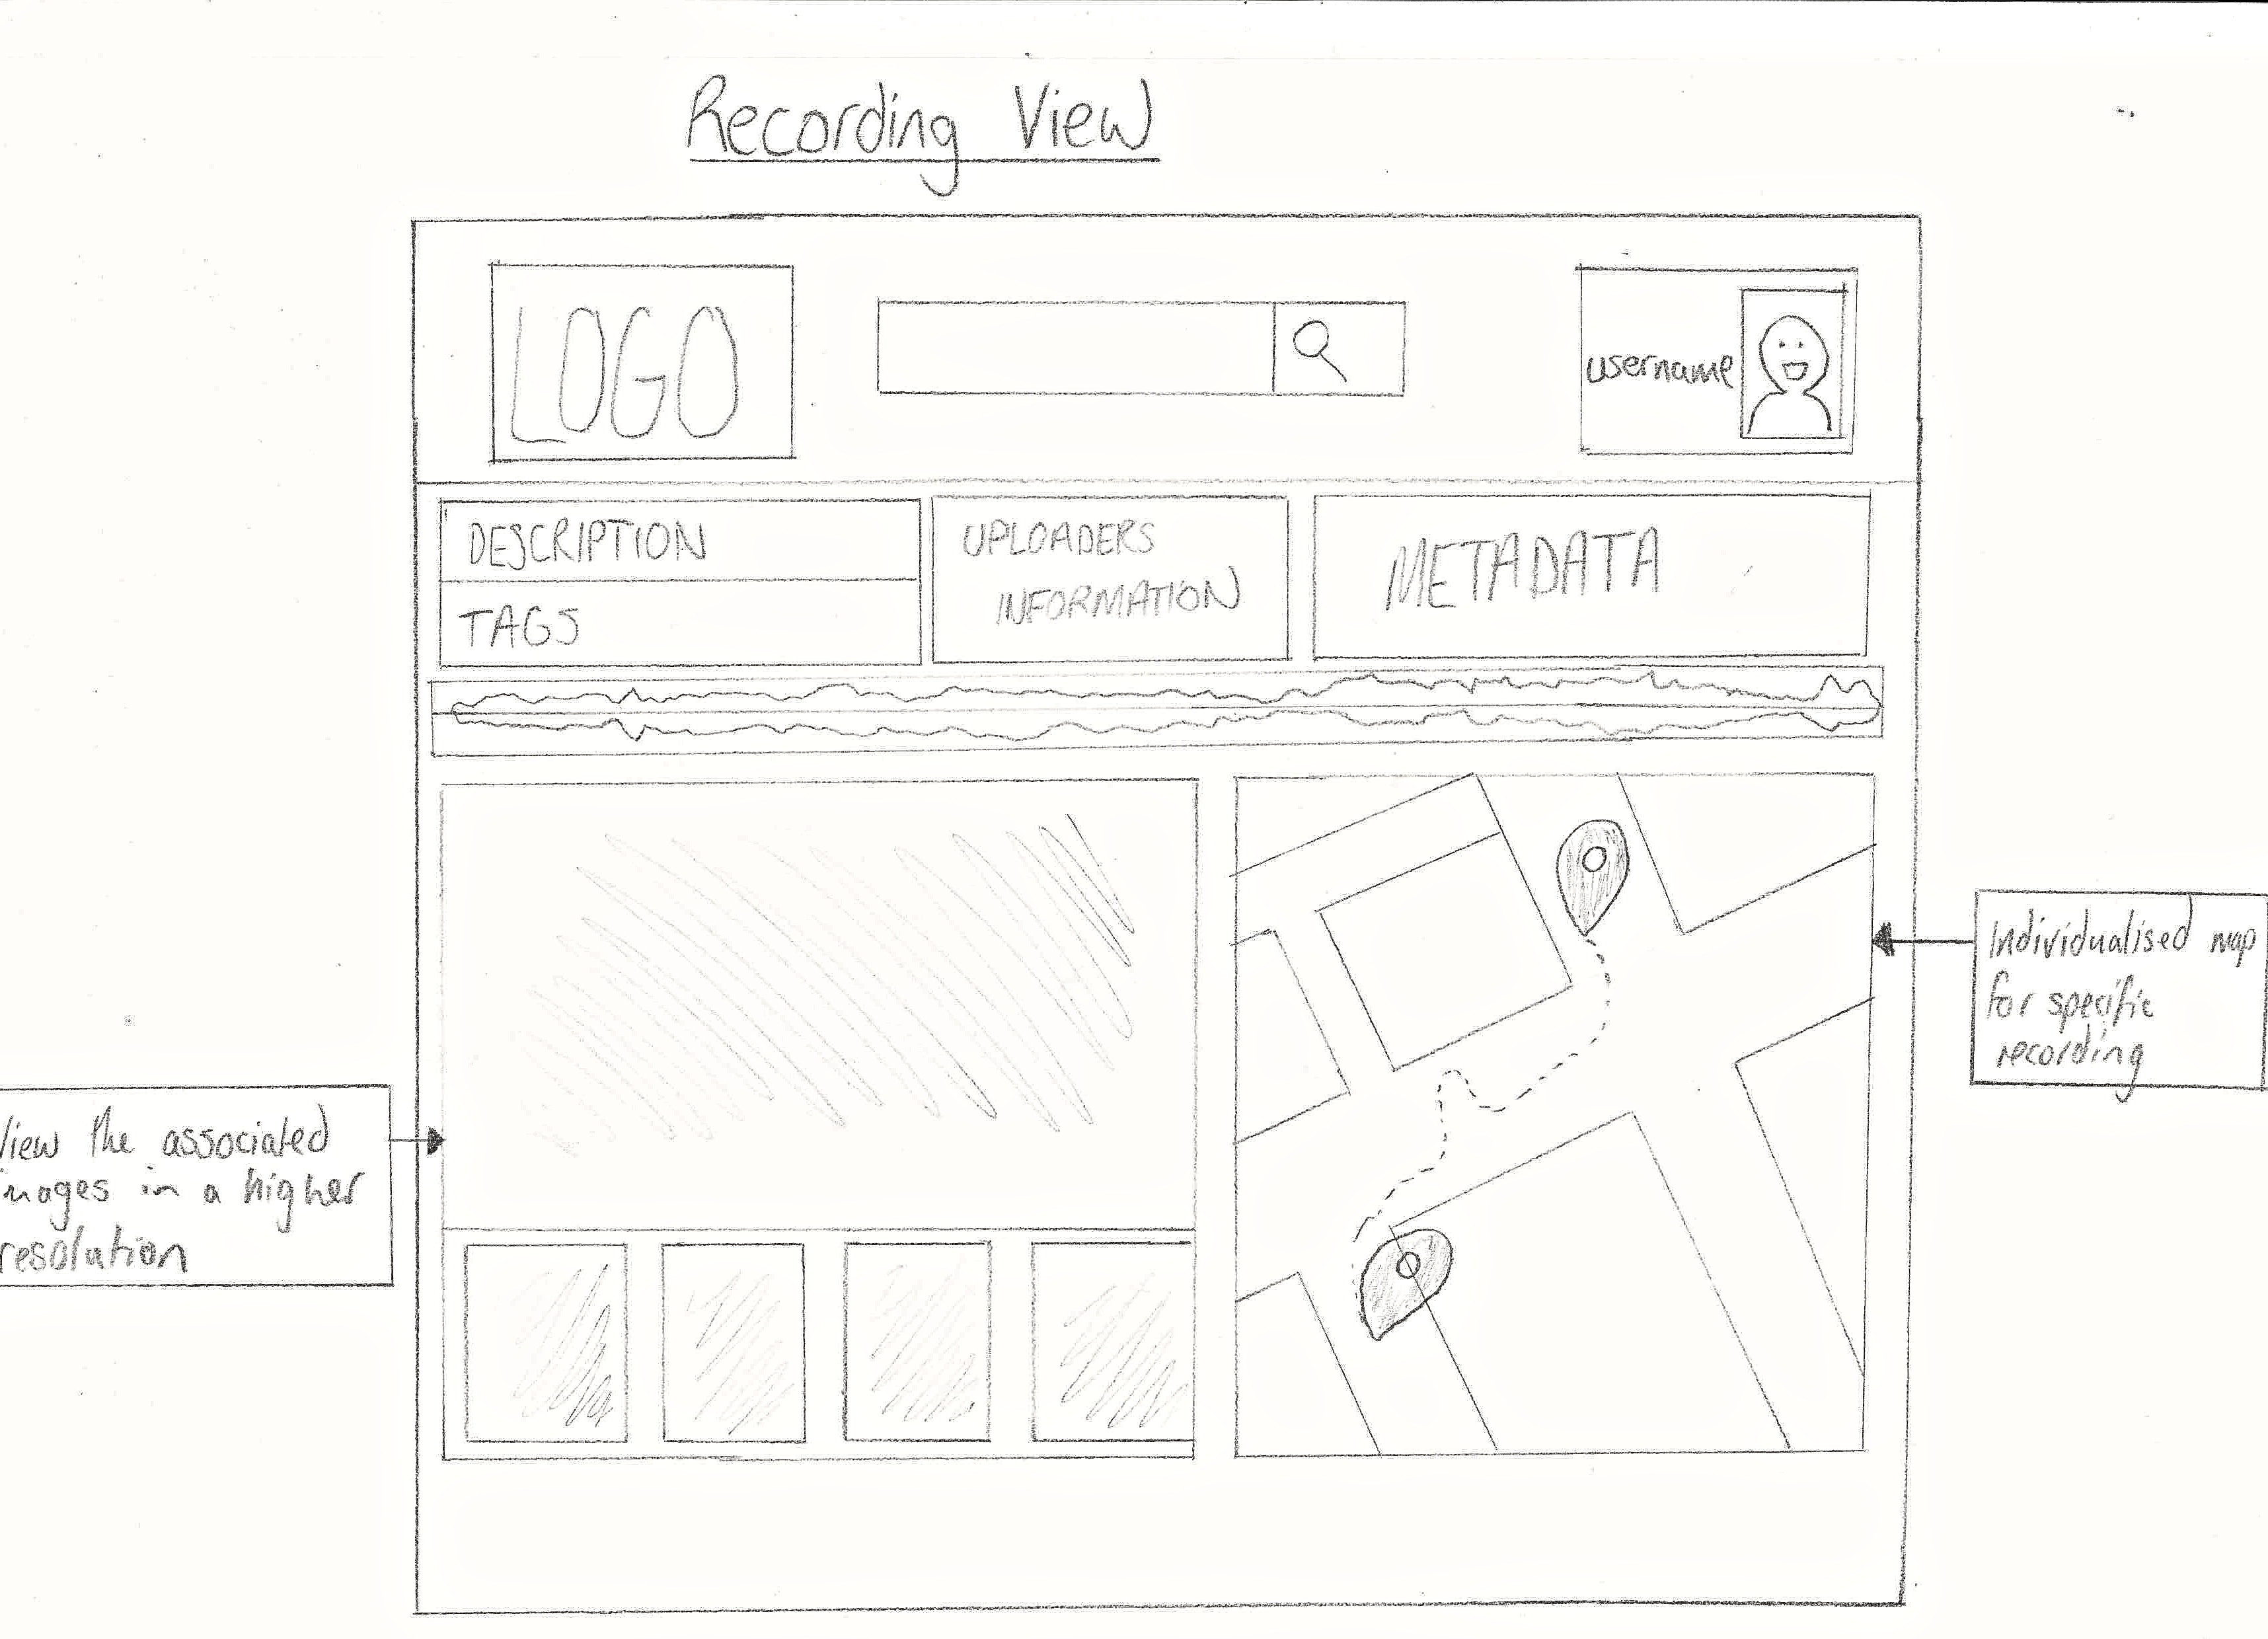
\includegraphics[width=0.5\textwidth]{images/web-recording-view.jpg}
\caption{Recording specific prototype for web application.}
\end{figure}

To accompany this main map view of MDRS was a user page which offered a
personalised insight into a user’s recordings and activity with the application.
It included a personalised timeline and map showing their personal contributions
to the map from which they could play, edit details or delete them from the
service. Along with all the other tools mentioned, the foundations of our
web application’s interface were laid.

\subsection{Android Application} It was decided early on to approach this
element of the project realistically and define a simple set of requirements to
make the application simpler to implement and make the user experience focused
on the core of MDRS, capturing information from the world around us. This meant
it was purely a capture and upload system and it wouldn’t be an alternative to
the desktop viewing interface for interaction with other user’s recordings. Our
focus made the application more achievable while leaving scope for extension in
future development for these playback features.

\begin{wrapfigure}{r}{0.35\textwidth}
\begin{center}
  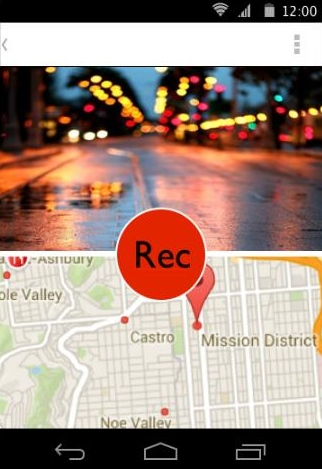
\includegraphics[width=0.34\textwidth]{images/android-digital-prototype-1.jpg}
\end{center}
\caption{Initial interface design}
\end{wrapfigure}

In developing an engaging user interface on Android devices, the team looked for
a scalable and intuitive design drawing influence from a wide range of
applications such as Foursquare, Snapchat and Google Play’s suite of
applications while consistently referring to Google’s Android Design Guidelines.
Foursquare was looked to for its integration of a map into a larger whole while
Snapchat’s unconventional, yet intuitive navigation model was seen as a strength
of the application while making an attractive UI. Google’s applications
portrayed the strength and beauty of clear typography and the undeniable rule of
mobile design where less is often more. A utilitarian minimalism through design
was the goal. The core functionality of the application was single use and the
flow through it was clear allowing for a relatively simple approach to be taken,
finding place for flair within the constructs the team placed on themselves.

INSERT INITIAL DESIGN PROTOTYPE HERE

This first UI design offers a split with both a map and view through the camera
lens. The influence for the central record button came from Foursquare’s
prominent placement of their check-in button, placing the key functionality
centrally to draw attention. Downsides to this were its limitations across
smaller screens and a confusing interaction model. Could a user interact and
capture an image before hitting record? This lack of clarity(dw) lead to a
revisionary second prototype.

INSERT SECOND DESIGN PROTOTYPE HERE

This prototype drew more influence from Snapchat’s sliding interface, replacing
its horizontal movement with a vertical one. Again showing the record button on
the divide between a map and camera view, once the record was initiated the map
would slide up bringing up the camera view which would reveal from behind a
frosted glass effect the user’s view into the world they were recording,
prompting them to capture images. This was found very visually appealing and
ended up mostly being used in the final application.


%==============================================================================
\chapter{Implementation}
\label{impl}

In this chapter, we describe how the implemented the system.

%------------------------------------------------------------------------------
\section{Web Application}

%Intro?

\subsection{User Interface}

When developing the User Interface we chose to use PureCSS for reasons
discussed in the research section.

It was the aim when approaching the User Interface to try and achieve
a consistent colour scheme and layout to make it as easy to use for
the end user as possible. Any unnecessary buttons were removed and
functionality was designed to be as intuitive as we could make it, as
opposed to lots of options.



\begin{figure}[ht!]
\centering
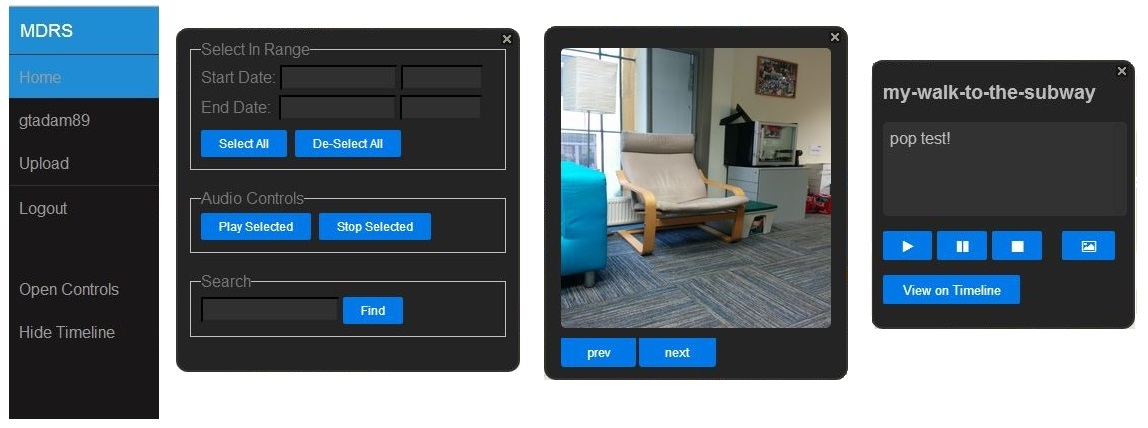
\includegraphics[width=0.95\textwidth]{images/ui-elements.jpg}
\caption{Navigation Menu, Control Box, Picture Box and Recording Box}
\end{figure}

\subsubsection{Navigation Menu}

The navigation menu came as a layout on the PureCSS website, it was
decided by the group that opposed to trying to create what has already
been created. We would use this layout and put our efforts into other
areas instead. Earlier on in the development all the UI controls were
located within the Navigation Menu, however it became quickly apparent
that this would leave it massively cluttered. So the controls for the
map were relocated to a separate box, and a button opening the box on
the page was located in the Navigation Menu.
\begin{figure}[ht!]
\centering
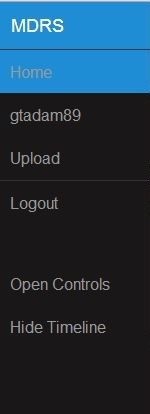
\includegraphics[width=0.15\textwidth]{images/nav-bar.jpg}
\caption{Navigation Bar}
\end{figure}
=======
map were relocated to a separate control box, and a button opening the box on
the page was located in the Navigation Menu. This menu also utilizes django's
user authentication system, so that if a user is logged in there username is
displayed on the menu item that would otherwise be named user. The current
page is also highlighted in the navigation menu, so as to cause the least
amount of confusion to the user. There is a button that allows the timeline to
be hidden, just in case more space is required due to smaller screens or just to
tidy it up.
>>>>>>> 4945247cbc128907a4986bbd12704fb038e19275

\subsubsection{Control Box}
The control box is separated into three logical sections; Select in
range, Audio controls, Search. If the Start Date is left blank within
Select in range it is assumed that all dates prior to the End Date are
desired. The opposite is true for End Date; and if both dates are left
blank all are selected. To create options for this could lead to a
more complicated UI though it proved unnecessary as this was intuited
by most people during testing.

JQuery Datepicker was used as the User Interface for selecting a date,
the colours were also edited to give a more consistent, and integrated
feel to selecting a date. Originally when a date was selected it came
up in the American format, though this was easily changed by modifying
the setting at initialisation.

It was decided to use JQuery Timepicker for selecting a time, this was
not integrated initially, however it was quickly realised that
datepicker on it's own was not much use for selecting recordings at a
similar time as it was far too wide a margin.
\begin{figure}[ht!]
\centering
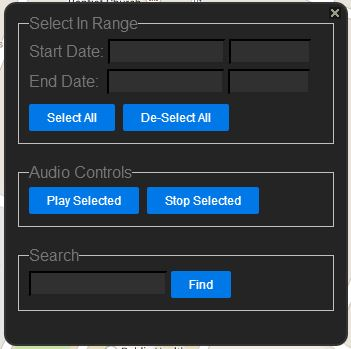
\includegraphics[width=0.35\textwidth]{images/ctrl-box.jpg}
\caption{Control Box}
\end{figure}
=======
It was decided to use JQuery Timepicker for selecting a time, this
timepicker has a similar appearance to that of the timepicker on google
calendar this was not integrated initially, however it was quickly
realised that the datepicker on it's own was not much use for selecting
recordings at a similar time as it was far too wide a margin.
>>>>>>> 4945247cbc128907a4986bbd12704fb038e19275

\subsubsection{Recording Box}
This box displays the meta data associated with the recording that has
been clicked. The colours chosen were picked to fit as closely with
the sites theme as much as possible. If the description is too long to
fit into to the description box it displays a custom  scroll bar. It
should work in most modern browsers though degrades gracefully if it
is not the supported. There are a number of buttons in this box each with
a separate purpose. The first three are audio controls for "Play",
"Pause" and "Stop"; they utilize buzz for playing the recording
associated with the record currently loaded in the box. The next button
is "View Pictures" which loads the Picture Box with the images for that
record.

\subsubsection{Picture Box}
The Picture box was kept as simple as possible with next and previous
buttons the same as the rest of the buttons in the user interface,
this box displays all the images associated with a recording. It uses
SlidesJS which is a plug-in for JQuery that allows you to view images
in a slideshow format.



\subsection{Map}

When creating
=======

\subsubsection{Map API}

The map API that was decided upon as discussed in the research section
was Google Maps.

The Google Maps API was used extensively throughout the development of
the home page with many of the Javascript classes and objects used. On
the Google Maps API website there was many examples given showing how
these could be used, these resources were invaluable during the
development process, especially during the early development process
allowing rough prototypes of certain features to be created with very
little trouble.

In order to create an instance of the map the class that was used was:
\begin{verbatim}
google.maps.Map
\end{verbatim}
There was very little that had to be changed in the code from the
simple example provided on the Google Maps website in order to create
the instance of the map, during the entire development
process. Bearing testimony to the simplicity provided from using this
API. There was only a few changes that were made to the way the map
appeared, such as removing certain UI elements that come with the map
as a standard. For example it was decided to remove "pegman" as we
would not be incorporating street view into our product and his
presence could prove to be an unnecessary distraction. This was done
using the object:
\begin{verbatim}
google.maps.MapOptions
\end{verbatim}
With the variables contained inside being set to the desired values.

After having created an instance of the map and it was styled
correctly, we were then able to receive the bounds of the map
displayed on the screen. this was called using the method:
\begin{verbatim}
getBounds()
\end{verbatim}
on the map object. This was important as from this we were then able to query our
database using JQuery (this method will be covered in a the JQuery
section) and receive from the database only the recordings that would
be currently visible on the timeline. For were we not able to receive
the bounds of the map and just all the recordings were returned, this
would prove a serious problem in scalability.

These recordings were then plotted on the map by creating multiple
instances of:
\begin{verbatim}
google.maps.Marker
\end{verbatim}
i.e. one for each recording. These markers must be created using this
object:
\begin{verbatim}
google.maps.LatLng
\end{verbatim}
This is the latitude and longitude of the marker, which is created
using the data that has been returned from the database. The data that
is used to create this object is the latitude and longitude of the
recording when it first started.
We decided to use a custom icon for the default marker to give a more
consistent theme, also in order to differentiate between non-selected
and selected markers a separate custom selected marker was used. This
was done by creating the object:
\begin{verbatim}
google.maps.Icon
\end{verbatim}
and passing it into the Marker class upon instantiation.

The behaviour of the markers had to be defined manually this was done
using JavaScript such behaviour was if the map was panned and a
recording fell outwith the bounds of the current view then this pin
would be removed, and then added back in again if it is brought back
in again to view. It was an initial requirement that support for the
\"selection\" of multiple recordings must be incorporated into the map
so that these recordings can then be played back in sync. What was
written allowed a pin to remain selected even if it was not currently
in the view of the map. In other words when a pin is selected it is
saved in memory until such time as it is deselected.

Originally the google maps infoWindow was used to display the metadata
to the user defined in the API as:
\begin{verbatim}
google.maps.InfoWindow
\end{verbatim}
however in the late stages of development this approach proved to be
inflexible as any minor changes to the appearance or positioning of
these infoWindow’s would prove to be overly complicated, for that
reason it was decided that when a marker was clicked there should be a
separate div component opened as shown in fig ?. Which in the long run
would hopefully save time and have a more refined appearance.

There was little debate as to how routes would be displayed on the map
as the only two options were to use:
\begin{verbatim}
google.maps.Polyline
\end{verbatim}
and the Google Maps Directions Service. However the Directions Service
could only make use of roads and paths, which quickly brings up
problems, for example if a recording is made inside a building or if a
route is incomplete on google maps. Polylines take an array of
latitude and longitude objects to create it along with any styling of
the line, this allows for a very accurate trace of the route taken,
even in unorthodox areas that may crop up; with a styling that can be
made to fit the theme of the website.

\subsubsection{Geolocation}

Getting the end users current location in order to use it as a
reference point for centering the map and displaying it with a blue
dot when they open up the webapp was achieved comparatively easily
with the use of the W3C Geolocation API with only a few lines of code
we were able to track the users current position by first checking to
see if the browser supports it (Which most modern browsers do) then if
so; create a new marker anchoring it at their location.
\begin{verbatim}
navigator.geolocation.getCurrentPosition()
\end{verbatim}

\subsection{JQuery}
JQuery only began to be fully used in the later stages of development,
this was largely due to having very little experience in it's uses
for development. However after completing a few basic tutorials on the
codeacademy website. It quickly became apparent how it could be used
to effectively and easily aid in the creation of an interactive
environment for the user.

The behaviour of the boxes including dragging, animations and visibility
in the User Interface are all controlled using JQuery. The inclusion of
JQuery to do this proved to be a great addition requiring very few
lines of code and little time in order to greatly enhance the end user
experience.

\subsection{Integration}

During the late stages of development there was a period of many months
where it was seeming impossible to integrate the timeline onto the same
page as the map. Thankfully however the problem was found to be with the
use of conflicting JQuery requests between the timeline and the
map. These get requests were:
\begin{verbatim}
$.getJSON()
$.get()
\end{verbatim}
Once this issue was found, there also proved to be a conflict withing
google maps aswell, and maps had to be removed from the timeline in
order to allow for full integration.


\subsection{Timeline (Implementation)}

In order to display the recording information in a convenient way for the end user, we identified the implementation of a timeline containing the recording objects as a key requirement for the MDRS project. This would give the team the opportunity to implement a user-friendly interface, enabling the user to easily switch between recording metadata and identify overlapping recordings in the database. After discussing and sharing our thoughts on the required specifications that we would expect from that component, we made a list of what it would display to the user. The recording metadata contains the following characteristics:

- recording duration
- recording start/ end time
- location
- ID
- recording description
- images/ photos taken while recording

After having clearly specified, documented and researched the functional requirements in order to try and find the best way to implement this key component for the system, we made design decisions and integrated it in the system. Having tested a number of different open source javascript implementations of different timelines, the final decision was based on the implementation differences and the degree of customization those products offered (all implemented in JavaScript):


- \textbf{SIMILE timeline} - http://www.simile-widgets.org/timeline/

- \textbf{Timeline JS} - http://timeline.knightlab.com/ (GitHub repository - https://github.com/NUKnightLab/TimelineJS)

- \textbf{Chronoline} - http://stoicloofah.github.io/chronoline.js/

- \textbf{TimeGlider} - https://github.com/timeglider/jquery_widget (moved here a year ago: http://timeglider.com/widget/)

- \textbf{Chaps Timeline} - http://almende.github.io/chap-links-library/timeline.html



\textbf{SIMILE}

<SIMILE timeline image> HERE

The SIMILE timeline (this product is implemented in javascript), is a very good example of an efficient and compact timebar able to accommodate a number of events in a relatively small space without looking too clustered with unnecessary information. It also supports scrolldown horizontal movement and  you can click and drag to navigate between objects using your mouse. However, there are a number of drawbacks associated with this open source implementation. To start with, its maintainability is poor - the last change that was made to the source code was in May 2009 which is very very long ago. We also researched the opinions of people who have tested it online and found out that there are mixed feelings regarding the SIMILE timebar. One of the issues people had experienced was memory leaks that were caused especially when dynamically loading and unloading events to the timeline. The poor maintenance of this product also had caused numerous people troubles with the implementation in different browsers as apparently there are many unidentified bugs that continue to increase with each browser update. Some people even had strange experiences of browser crashing as a result of using SIMILE (more information can be seen in this StackOverflow topic: http://stackoverflow.com/questions/4700419/alternative-to-simile-timeline-for-timeline-visualization). Customisation and updates are also very difficult considering the relative lack of documentation or poorly documented code segments which was also one of the main reasons why we decided that it will not be the most suitable option for what the user interface requires.


\textbf{Chronoline}

<Chronoline timeline image> HERE

The Chronoline timeline was also a very attractive alternative and it is really compact indeed. However, for the purposes of the multi-device recording system, it looked too simplistic and did not provide enough options for further customization in order to make it work as we would require. It also does not support mouse dragging when switching between the recording objects. After a thorough research we discovered a number of people that were having issues with this timeline as well and, although it is indeed a well maintained project, its documentation is poor.


\textbf{Timeglider JS}

<Timeglider JS timeline image>

Timeglider JS was an option which really captured the attention and took some time to test in order to see whether it would be a good option. It supports many features and has a number of sub-components however they were making it a little bit too complicated for what we actually needed and it looked kind of too demanding for the average user as it required some time to get used to and understand how to interact with it. This product is clearly documented, containing detailed information on how to use the API to customize it on the website which was created about a year ago when the code from the GitHub repository was transfered to timeglider.com. After carefully considering this option, we decided to continue searching before making a final decision.


\textbf{Chaps}

<Chaps timeline image> HERE

The Chaps timeline, is also really impressive - not very heavy and at the same time, not too simplistic for what we needed. It supports mouse scrolling for zoom-in / zoom-out and mouse dragging in order to slide it horizontally as most of the other alternatives. It was also one of the viable options which we left to the side before making our final decision. However, when considering it, we noted a not very serious, but still significant drawback, which was easily fixable - it does not look very elegant and is not very dynamic, not allowing the user to switch between the objecte using left and right horizontal arrows. In addition, its structure would not suit very well with the rest of the user interface.


\textbf{KnightLab Timeline JS}

<KnightLab Timeline JS timeline image> HERE

Last but not least important candidate - Timeline JS. This product is well maintained and has an active community contributing to its GitHub repository (https://github.com/NUKnightLab/TimelineJS), making it very user friendly and easy to test. It looked like a really flexible and customisable solution right from the start, but this needed to be verified after testing the product’s functions. Timeline JS is coded in javascript, CSS for styling and some python is used too.

One thing which really distinguishes it from the rest of the candidates is the fact that it is thoroughly documented in the repository as well as the website. And everyone is welcome to ask questions on their community forum, make changes or suggest some alterations to the code in the GitHub repo by opening new tickets for enhancements or bug fixing. We had some questions for the json template as we intended to use this format to dynamically feed the timeline with information extracted from the database and contacted their team. They responded quickly and gave us all the answers we needed (community forum: https://knightlab.zendesk.com/forums/22551396-TimelineJS) so this proves how well maintained this open source software is and made it even more attractive. It also provides simple and easy interaction when used from a mobile device such as a smartphone or a tablet, or any other touch-screen device.

Timeline JS also provides a number of customization options which are clearly documented on the website and it has a nice display field for which could be using for the recordings’ metadata. The interface is extremely responsive and provides an elegant way of switching between recordings’ information either by clicking a recording object or by using the provided left and right arrows for horizontal sliding. What is more, it has a bookmark built-in function which allows for recording object to be easily linked by using the format - #number - a hash tag followed by the recording id which would definitely prove useful at a later implementation phase. On top of that, we thought that being able to specify the exact starting point for the objects on the timeline was another huge benefit.

After comparing timeline JS with the other viable options and having contacted their representatives or making research on other people’s opinions all over the internet, we were ready to make the final decision of the implementation to use. The fact that many developers, who were looking for an elegant and easy to customize, well documented, and clearly structured open source project easy to feed with dynamically generated json, after trying various different options, had discovered that Knight Lab’s Timeline JS works best for them, made us confident that choosing it would be the right thing to do. And so we did.

MORE TO ADD HERE//



% - - - - - - - - - - - - - - - - - - - - - - - - - - - - - - - - - - - - - - -
\subsection{Server and Django configuration}

At the outset of the project the team had planned to build two independent platforms, one back-end server used to process audio and a separate client application to view and amend data. However the team took time to discuss the positives and negatives of this approach; the result of which was decided this was not the most sensible solution.
The team supervisor suggested we look into Django as a all in one solution, as it provided many of the features this project includes and the team would also benefit from using a simple and also familiar language like Python.
To be more specific, Django provided the team with built in user authentication, a reliable and easy to use model view controller structure, full database support and integration with the application and the simple fact Django is a web application framework allows the application to be used across almost any device without much regard of portability.

With this decision made a GitHub repository was made and a skeleton Django project was set up. No-one on the team had used Django before however all members were experienced in Python. A little research was done and a series of tutorials entitled “Tango With Django” was discovered.
Upon seeing the clarity and level of detail of this document, it was decided to use this as a reference with which to build the web application.
Team members were given chapter numbers to reach by deadlines; however these were not always met by all team members. The team made good progress in learning and understanding how to construct a Django application correctly.
Once everyone was familiar with the process and details of the Django framework tasks were dealt out and members of the team were expected to achieve certain levels of work each week. However it became quickly obvious that many parts of the application relied on others, meaning one member’s work would be held back while another finished theirs. This held back productivity in certain areas of the application, certainly when involving the database and the models associated with it.

Progress with the web application was steady, the back-end was actually a fairly simple affair in comparison to the front-end which was heavy with scripting.
Back-end scripting mostly involved getting the models to suit what was needed correctly, it took several trial and error attempts however once the team managed to work out the correct collection of models it was mostly left alone. The only real issue the team ran into was some of the audio formats in the later stages of the project. At the outset OGG was decided as the format to use as it had a great compression to quality ratio; however it was discovered that Android could not, in fact, encode audio to OGG directly. Since a majority of the web code had already been written a decision was made to simply take a format Android could encode in and then convert it to OGG upon upload to the server.

%More added later

%------------------------------------------------------------------------------
\section{Android Application}

\subsection{Early development} With little experience in developing for Android, our aim was to take the most key requirements and create simple demos of each aspect. Then taking all the basic knowledge gained from this process, create an application with the must have features, structured in a way to allow further development if time constraints allowed.

\subsubsection{Learning Resources and Tools} Google's Android tutorials served as an early touchstone in development, offering an understanding of an application's structure and layout in development. These go into great depth about most of the classes and APIs useful to MDRS but often this depth was made them inpenetrable. For example, you can either implement an interface for an Activity though your Activity's .java file programmatically or in a separate layout .xml file. Google's tutorials would switch between these methods, muddying the team's understanding of how to work in this new development environment while adhering to good code standards.

Other learning resources were scarce and when found usually weren't to a good enough standard to be useful. This meant that alongside Google's tutorials, Stack Overflow was the main resource used to aid development. This crowdsourced Q&A service served invaluable in fixing bugs and explaining topics. The answers far exceeded the quality found in some textbooks that were used. Twitter also served as a direct communication to the development community with advice and encouragement coming from other Android developers.

As development began, an early decision made was to askew the use of Google's new Android Studio to use Eclipse with the ADT (Android Development Tools) plugin. This reduced the number of new tools to learn and avoided using unstable software while trying to learn a new SDK. All of the development was done on personal devices due to the University's lab machines not having the required software and refusal from technicians to have it installed in a useful manner. This limited development time as it had to be carried out almost exclusively at home in off-hours. It also limited the chance of gaining any help from other student's insights to solve common issues in Android development. Overall poor access to tools caused extensive issues in the protracted  development cycle.

A Nexus 5 and Nexus 7 (2012 model) were used as testing devices. As Google designed models, the Nexus range are a good standard for development as they run a clean install of Android on common hardware shared across the device ecosystem. This reduced the amount of testing required and avoided troubleshooting vendor specific errors or bugs. These devices also allowed the UI/UX could be tested on varying screen sizes to see how it reacted. As testing expanded, the application was also later tested on an HTC One and a Samsung Galaxy Note.

\subsubsection{Audio Recording}    Audio recording is key to MDRS' premise so was the first thing to be implemented. Through our learning resources the MediaRecorder class was chosen to implement this functionality. The alternative to this was AudioRecord. This class captures the raw bytes of audio data which allows for much more control over processing and format choices but at a higher degree of difficulty. External Java libraries would be required alongside a more complicated implementation making MediaRecorder the simpler choice while still meeting our needs.

Prototypes were rapidly built referencing various tutorials. However these prototypes repeatedly ran into complex issues and consumed an extensive portion of development time available. MediaRecorder would consistently crash the test devices with little debug information given by the error logs. Testing was further slowed down as MediaRecorder doesn't work in the Android Virtual Machine availble. This meant all testing was done on devices, complicating the entire process. Combined with poor understanding of the Android SDK these tests caused many issues and took up all Android development time between Mid-November and late December 2013.

Eventually through extensive research surrounding MediaRecorder and learning more about debugging Android code, the main problem was found to be in interacting with external storage and the dichotomy between truly external storage, such as a removeable SD Card, and internal-but-external storage. As vendors moved to add internal storage in their Android devices, the OS would still recognise that as an external source compared to ROM on the chipset. This means that while it is internal, the OS views it as external. By creating a /textit{Catch-22}, it made it difficult to access the correct storage in which to place MDRS' data. With this problem found, the issue was resolved and development continued.

\subsubsection{Google Play Services}    The next thing to integrate was the Google Play Services library. This gives Android developers extensive access to many of Google's services. For MDRS, the interest was soley in the Maps and Location APIs. Integrating this library into the project rasied multiple initial issues. While adding a library should be a relatively simple task, there were wildly varying instructions on how to do this, leading to a lot of confusion. While it is possible to link it to the build path by manually downloading the library and then linking it using Eclipse, other instruction sets described the use of Apache's Ant or Maven files to decalre the dependencies. In practice however these didn't work reliably. In the end it was decided to store the library locally in the project's repository. This led to an issue with the IDE. Eclipse stores the full path to the library's folder on the computer statically instead of just its path inside the current workspace directory. This meant when switching between development environments (Windows and OSX) that it had to be manually updated. Once these dependency problems were resolved development quickly continued to the implementation of Maps.

For MDRS we required two map views, one as the main point of interest on the start screen and a second in the upload screen indicating the path their recording took with a start and end pin. These relatively simple requirements meant a lot of the code required could be reused from Google's example applications. The code required was relatively short but by using Play Services there was a lot of boilerplate code needed to check that it was installed on a device and to connect to Google's servers. A series of small tweaks were made to the default map, removing certain UI elements and changing the zoom levels. This manifested the team's first experience of inconsistency between devices. When running on a Nexus 5, the 'Show my location' button, despite being explicitly declared, didn't appear while the same build of MDRS running on an HTC One did show the button.

The main issue that was found with the implementation of Maps was a bug which crashed the app if it was opened before another application using Google Maps had been opened on the device. While puzzling and initially demonstrating an erratic manifestation pattern, the problem was found to be referencing the device's last location, using getLastLocation(), when it didn't have one passing a null value and crashing the app.

Placing the map into an activity's layout was done by referring to a map fragment element which was then initialised programmatically. This displayed the benefits of Android's flexibility. Where initially having the option to programmatically do the layout or use XML was confusing, in this case it allowed the map to be placed in XML then modified in code. This made populating the map with pins and other markers a simple call of a method and feeding in data from the Location API.

While Android has its own Location classes, the Play Services' API was chosen for its higher level abstraction and excellent learning resources. While Android only had the reference documents, Play Services' was accompanied by tutorials and getting started guides. This sped up development, saving the a lot of time researching for good learning resources. Making use of the LocationService and LocationManagers allowed the application to gather information from the device's GPS module or the next most accurate source of positional data. This was then stored in a LinkedHashMap. Using this data structure allowed the Location objects collected to be stored in a chronological order with their timestamp acting as each object's key. Parsing this information into JSON later in the upload process was trivial due to this structured approach at the data capture stage.

\subsection{Main Development}
\subsubsection{Application Restructure}
With these prototypes and test applications complete and the advent of the new year, the previous codebase was scrapped in early January. This fresh slate streamlined any previously written code and allowed a rethink of the structure from previous plans. While the application was originally going to be a single activity which would dynamically change, research showed this to be completely wrong. An activity as defined in Android is:

\blockquote{An Activity is an application component that provides a screen with which users can interact in order to do something, such as dial the phone, take a photo, send an email, or view a map. Each activity is given a window in which to draw its user interface. The window typically fills the screen, but may be smaller than the screen and float on top of other windows.}

Taking this into consideration the app was broken into three key stages, a start screen, recording and upload activity. This separation of concerns made the code more readable and easily understood. As development continued and more external classes were used and while not activities were included in the 'src' directory it could be seen that, while three activitys was better than one, a lot of the code required for the three main views the user had of the app could be separated into their own '.java' files to make the code much easier to understand but by this point there was not enough development time to refactor the entire application.

PLACE UML DIAGRAM OF APPLICATION HERE

\subsubsection{Modifications to Existing Features}
To begin, the maps and location tracking features were extended. The ability to plot a recording’s path on a map was developed using the excellent Google Maps APIs documentation available. This was used on the final upload screen, giving a sense of the journey travelled. Improvements to time keeping were also attempted. The inclusion of an external Java library which could import SNTP time was hoped to be used. The Simple Network Time Protocol is designed for simplified access to nuclear time servers where sub-nanosecond accuracy is unnecessary. Ultimately due to time constraints and restrictions on modifying an Android device’s system time, the time from GPS was relied on. While less accurate still gave sub-millisecond accuracy which was satisfactory for our uses. In addition to retrieving time stamps and Latitude and Longitude, the Location object also offered the orientation of device. By passing all of this information along, it offered the project scope for stretch goals such as an immersive exploratory street view if development finished early.

The MediaRecorder implementation was also modified to use AAC compression instead of the originally planned OGG. This offered higher quality audio fidelity while keeping a small file size for efficient upload to the web application.

\subsubsection{Image Capture}
As a modification of the original specification, the team had added capturing images as a must have requirement to allow the user to create a richer experience to share on the web application. As a core requirement of our application, this was the next feature to be implemented in MDRS Mobile. With Android there are two methods of capturing images within an application. An app can send an intent to the OS, taking the user to their default camera app with which they can take an individual image. The user will then be taken back into the original application with the image in hand. This simple approach is useful if capturing individual images. For MDRS Mobile this would be an unintuitive approach. Every time the user tried to take an image they would have to wait for the app to safely send the audio and location capture to an asynchronous background thread and then wait for the camera application to load. Depending on the device, this was found through testing to take anywhere between 2 and 10 seconds. To avoid this, the application uses a custom written ‘Camera Preview’ which allows a fragment to be embedded within the interface through which to see a device’s camera view. Surrounding this it was necessary to add a button to capture images. In initial implementations this was a separate button. This allowed for easier testing. A major problem found while putting this functionality in place was saving the file while still allowing the user to capture more images. The asynchronous thread dedicated to saving the file would become overloaded with requests to save. To solve the problem, while giving the user a visual indicator of successful image capture, a 3 second ‘freeze frame’ was put in place. This gave the thread enough time to save the image while letting the application continue capturing images at the user’s request. As development of features finished and UI/UX corrections were made a transparent ImageButton was placed over the camera preview and the visible button was removed. Users could tap anywhere on the screen while recording to take an image and continue their recording without interruption. This functionality is communicated to the user through an on screen prompt as they start recording.

\subsubsection {Data Processing and Upload}
Once the user has completed their recording, they are brought to the upload screen. Here all the information gathered is prepared and bundled for upload to the server, either manually or using the mobile connection/WiFi. The AAC audio file was sent uncompressed for processing by the server. The location data gathered and stored in the LinkedHashMap was stored in a JSON file for transfer. A title and description were also gathered for storage in a JSON file. This was done using the built in Java JSONArray functionality with the native FileWriter to write it on the device.
(FOOTNOTE - ALL DATA WAS STORED IN AN INDIVIDUAL FOLDER WITHIN A MASTER MDRS FOLDER ON EXT. STORAGE DENOTED BY STARTTIME)
With the high resolution of images being captured, compression was essential for transfer of these files. While Apache’s Common Compression appeared to be the most used library to create .tar.gz files, the team opted for JArchive. This library serves as a wrapper to Apache’s work, simplifying the creation of an archive significantly. Implementation of these JSON and archiving was quick due to the clarity of their associated documentation. While the libraries used were not the most feature complete, their simplicity was the key to faster development on an already tight schedule.

With a ‘should have’ status, the ability to upload directly from the device was one of the final features to be implemented. After research, (INCLUDE LINK)Android Asynchronous Http Client was chosen. This library is used in applications ranging from online multiplayer games to Instagram. It is a great option for efficiently transferring data to and from servers from within an Android application. It’s continual development and widespread use made the support surrounding it easier to find. This again was easily implemented within the application, supporting direct upload from the application to the web app. Unfortunately the server side processing could not handle POST requests from the app. This was found out at an extremely late stage in development. Alternative implementations using (INCLUDE LINKS!!) Square’s okhttp and Retrofit libraries and Apache’s Java HttpClient were attempted to alleviate the issue. These offered no better results and with no time to refactor large sections of the Django back-end, this feature had to be left written but unsupported.

\subsubsection{Aside}
Another feature which the team tried to implement was background recording. To make a truly useful application, it would have to let the user conserve their battery life by being able to turn their screens off while still capturing audio and location. They could then reopen the app to capture images as and when they pleased. An extensive amount of development time was dedicated to this ‘should have’ feature. Unfortunately this was attempted in the middle of development and, again, time constraints limited the team’s ability to refactor large amounts of the application to make this work. Many parts would have needed completely rewritten. This feature was dropped in favour for completing the key requirements.

\subsubsection{Finishing Touches}
With all the needed features implemented, the last development work required was refinement of the UI/UX. With the help of an external graphic designer, new graphics were produced for the recording button and a new logo was developed from the team’s original designs. Working with the XML layout files was a frustrating experience, requiring a lot of patience. To enhance the upload screen a gallery of the user’s captured images was implemented. This view was horizontally scrollable to allow the user to check all their images before upload. In the original prototypes, it was hoped the user could dismiss these with a swipe but this was unimplemented in the final application.

Overall, the application met the must have requirements desired while offering an easy to use and attractive interface through which to use it.

%==============================================================================
\chapter{Evaluation}

We evaluated the project by...

%==============================================================================
\chapter{Challenges}
\label{Challenges}

A number of the challenges we encountered were through a lack of previous
experience and inaccurate expectations held by each member of the team. The
development process offered a lot of flexibility in finding weaknesses in our
ideas and restructuring them forge better working practices and develop new
insights into the workings of a small scale agile team.

\subsection{Communicational}
Our main communication issues was the over-complication and over dependence on multiple services for specific channels of communication. This diffused each team member's attention, turning a lot of communication into asking where other information was kept instead of working on the project.

As previously described we embarked on the project with the intention of using a Redmine instance to keep track of project details, GitHub as our VCS and Facebook for communication. This convoluted mix made it near impossible to keep track of discussion about specific issues and problems.

Our success with Facebook as a means of communication was varied. Its IM service was excellent allowing the team to communicate about the project as a group or one-to-one. Facebook's mobile applications made this easy to access while in transit which was an added benefit for those who commuted.

The Team's group page however was wholly unsucessful in our desired use case. The main point of weakness was the lack of chronological discourse of our messages. This meant you might have to scroll past a dozen posts to get yesterday's discussion just because it wasn't the most commented on post. The page's bloat UI also made it difficult to navigate with no search function to quickly find an old post quickly. While its feature which tells you who in the group has read the post was useful, the rest of the functionality was subpar.

At the outset, Redmine was easy to set-up and seemingly simple to use. However it became quickly appaerent this tool sees it's uses in far bigger, more indepth projects.
Redmine allows for depth and breadth for a large scale software solution. It's built in wiki, GitHub intergration, news feature and outstandingly detailed issue tracking were simply overcomplicated and bloated for our uses.
The team used the platform for at least a month, religiously creating issues correctly and handing them out. It was only after a large number (at least 60) issues with sub issues were created that it became blindingly obvious Redmine was simply dragging the entire project back.
A second, large, issue was simply the disconnection from GitHub. Redmine boasts a GitHub intergration, however this is little more than an output of the latest commits and a diff view; offering none of the excellent tools and views GitHub offers.

Through other project work and happenstance, the team discovered GitHub's issue
tracker and wiki features which are individual to each repository. These quickly
became the default means of tracking progress for MDRS, replacing Redmine. The
customisable labels and ability to cross reference issues from commits were
invaluable. GitHub's fast and responsive web interface scaled well across
devices and meant everyone was able to be involved in decisions and contribute
issues to work on. Most of all it succeeded due to the team members being on GitHub to check commits of various projects and to collaborate on other projects. Whereas Redmine required an intent to visit it and keep up to date, GitHub just merged this information into an efficient user experience that had become a daily destination for the team during their work.

Surprisingly email notifications became a great source of information. As
default, GitHub sends out emails for every comment or new issue created. While
filling up inboxes, this device agnostic communication platform made for great
commute reading. While notifications can easily be lost in a endless-scroll, a quick glance at the subject line would keep each team member up to date instantly. The
emails were also small, actionable pieces of key information to keep track of the
project's direction as a whole.

We also found by replacing web-based interaction with face to face communication improved our productivity immensely. Even a quick 2 minute conversation could convey the same information a 20 minute IM chat could. While each team member kept their own schedule, we always took advantage of these conversations to keep one another up to date.

In future, due to the distributed nature of the team and constantly shifting
focus of attention for different deadlines, the team would leverage email more.
Weekly status reports would serve as talking points to hopefully make meetings
more productive, giving members time to prepare their thoughts. These would also
serve as evidence of communication and would be easily accessible at a later
date in a chronological order. While the agile principles can definitely be applied to a distributed workforce, using the methodology when the team cannot focus on one project for an extended period of time, in our usage, does not work. Switching between various projects and deadlines meant agile was reduced to agily moving between disciplines to complete the most important task to create a better end product.

\subsection{Technological}
Most technological issues revolved around a lack of experience and knowledge at
the beginning of the project. Issues such as handling dependencies with the package management system \textit{pip} with, initially, no requirements.txt file made setting up a new virtual environment a challenge. Everything had to be manually installed allowing for greater risk for failure and variation between team member's development environment. Our ignorance regarding virutal environments also made maintaining consistency harder throughout development. After working on Django development using /textit{Tango with Django}, the team studied and began to use virtual environments to simplify development. Until resolved, these issues caused a lot of problems for certain team members.

Another major misunderstanding came with the team using our version control system, git. If used correctly, git allows each developer to work on their local machine, testing and committing any changes to the repository. In our case this should have then been pulled on the server, effectively 'deploying' our changes. Initially we were all using SSH to access our server and then working directly in the terminal, creating conflicts and locking file issues. This was quickly resolved when the team researched the issue, quickly changing to the correct workflow.

\subsection{Organisational}    At the beginning of the development cycle, agile roles were assigned for scrum master, communicator with supervisor, librarian and developer. Throughout development these roles merged and adhered to the agile principles even further. Due to the ad-hoc nature of the development team and shifting focus amongst projects, a different team member shifted into the scrum master role. This team member handled all secterial jobs such as keeping minutes at supervisor meetings and assigned each team member tasks in a bid to keep to the work schedules. These tasks were assigned taking into consideration each team member’s strengths and interests. This increased productivity within the team, pushing our development further and allowing us to expand on the feature set included in the final project.

%==============================================================================
\chapter{Future Work}
\label{Future Work}

Throughout development, a number of compromises and mistakes were made due to inexperience and limited development time. In retrospect, the team has acknowledged and recognised a number of improvements that could be made to the project as a whole that could be worked on in the future.

As modification to the project’s central vision, the team would include search as a key feature. While the current project’s timeline and map offer a unique way to explore the recordings, this wouldn't scale well to thousands of recordings. Integrating search engine alongside the introduction of tags would improve a user’s experience. Hopefully it would spur an users to stay on  the website for longer. They would be able to explore all the recordings better and find more relevant content. Ultimately MDRS could produce large sets of data and not integrating a proper  search functionality would be detrimental.

With the integration of these features to the web application, the user interface would have to be rethought. The use of a responsive framework such as Twitter’s Bootstrap or Zurb’s Foundation could offer a streamlined interface and improved interaction models. The team would also make changes to the timeline feature. While TimelineJS offered a flexible model, recent research has shown that we could have taken advantage of Django itself to more efficiently populate and render the timeline in our web application. This refactoring would greatly simplify our current codebase and improve performance significantly. The team have also recognised that giving users options to log into MDRS through existing social accounts (through systems such as OpenID) would be beneficial and smooth their introduction to the system as a whole.

The team would also hope to use the orientation data being pulled from the Android device to create an enhanced ‘Street View’ that, when viewing an individual recording, could display the recorder’s perspective as they moved and overlay their images on top of Google’s Street View imagery. This innovative perspective would help further differentiate MDRS from its competitor, offering a unique comparison of the constantly changing state of our cityscapes, depending on events or times of year.

The Android application would ideally be completely rebuilt. While the current iteration meets most of our functional and non-functional requirements, it has fundamental flaws associated with the severely limited development resources. Login with Social Auth would be integrated and background recording would be a must have feature from the beginning.

%==============================================================================
\chapter{Conclusion}

A great project!

%==============================================================================
\section{Contributions}

%Wasn't this written somewhere?
Conclusion here

%==============================================================================
\bibliographystyle{plain}
\bibliography{example}
\printglossaries
\end{document}
